\documentclass{standalone}

\usepackage{pgfplots}
\usepackage{tikz}

\begin{document}
\pagestyle{empty}
	
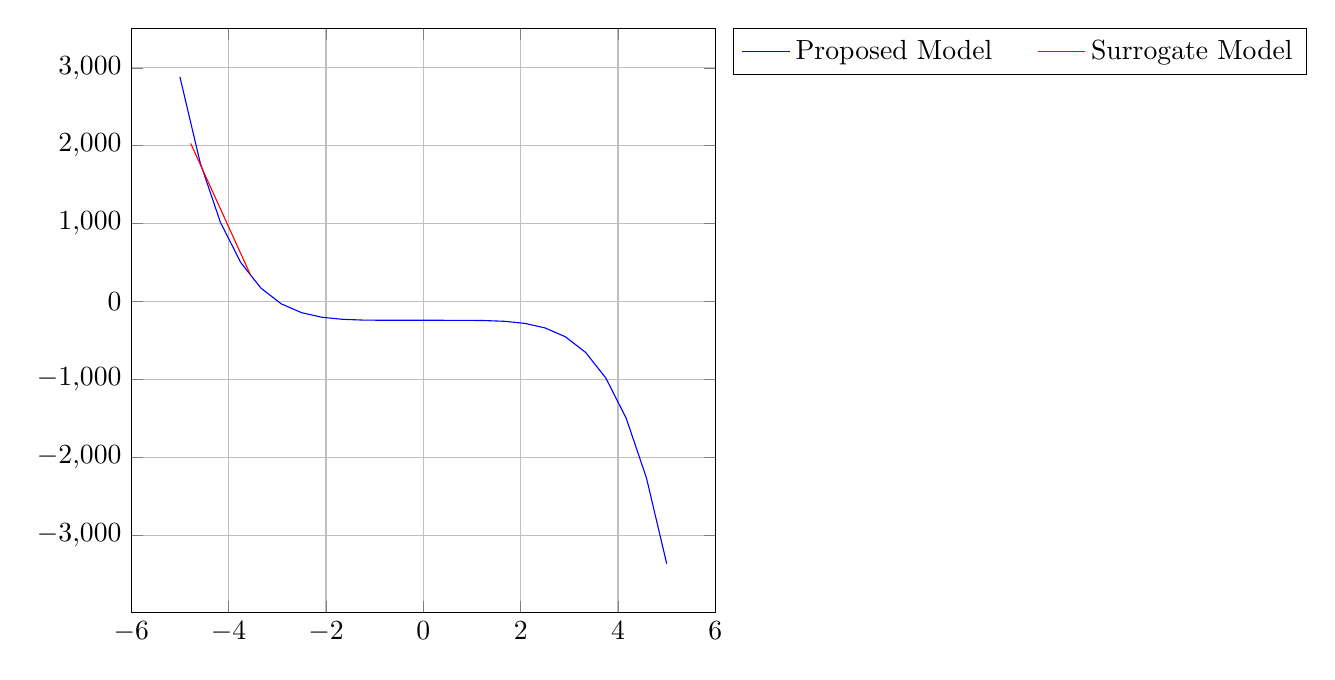
\begin{tikzpicture}
	\begin{axis}[
		height=9cm,
		width=9cm,
        grid=major,
		legend pos=outer north east,
		legend style={/tikz/every even column/.append style={column sep=0.5cm}},
		legend columns = 2,
	]
		
	\addplot [blue, mark=none] {-x^5 - 242};
	\addlegendentry{Proposed Model}

	\addplot [red, mark=none] coordinates {
		(-4.77778,2027.60977)
		(-3.55556,347.84069)
	};
    \addlegendentry{Surrogate Model}

	\end{axis}
\end{tikzpicture}

\end{document}